\documentclass[]{article}

%opening
\title{4M24 CW - High-Dimensional MCMC}
\author{Candidate: 5562E}

%packages
\usepackage[margin=0.5in]{geometry}
\usepackage[export]{adjustbox}
\usepackage{mathtools}
\usepackage{graphicx}
\usepackage{amsmath}
\usepackage{amssymb}
\usepackage{hyperref}
\usepackage{caption}
\usepackage{subcaption}
\usepackage{parskip}
\usepackage{listings}
\usepackage{pdfpages}
\usepackage{bbm}

%package setup
\graphicspath{{./img/}}
\DeclareMathOperator*{\argmax}{arg\,max}
\DeclareMathOperator*{\argmin}{arg\,min}

%custom commands
\newcommand{\Fcal}{\mathcal{F}}
\newcommand{\idft}{\mathcal{F}^{-1}}
\newcommand{\Xcal}{\mathcal{X}}
\newcommand{\Ncal}{\mathcal{N}}
\newcommand{\Acal}{\mathcal{A}}
\newcommand{\Bcal}{\mathcal{B}}
\newcommand{\cmplx}{\mathbb{C}}
\newcommand{\Lcal}{\mathcal{L}}
\newcommand{\Mcal}{\mathcal{M}}
\newcommand{\indep}{\perp \!\!\! \perp}
\newcommand{\iid}{\stackrel{iid}{\sim}}
\newcommand{\figwidth}{0.4\linewidth}
\newcommand{\betaml}{\hat{\beta}^{ML}}
\newcommand{\Expect}{\mathbb{E}}


%section numbering
\renewcommand{\thesubsection}{\alph{subsection}}

\begin{document}

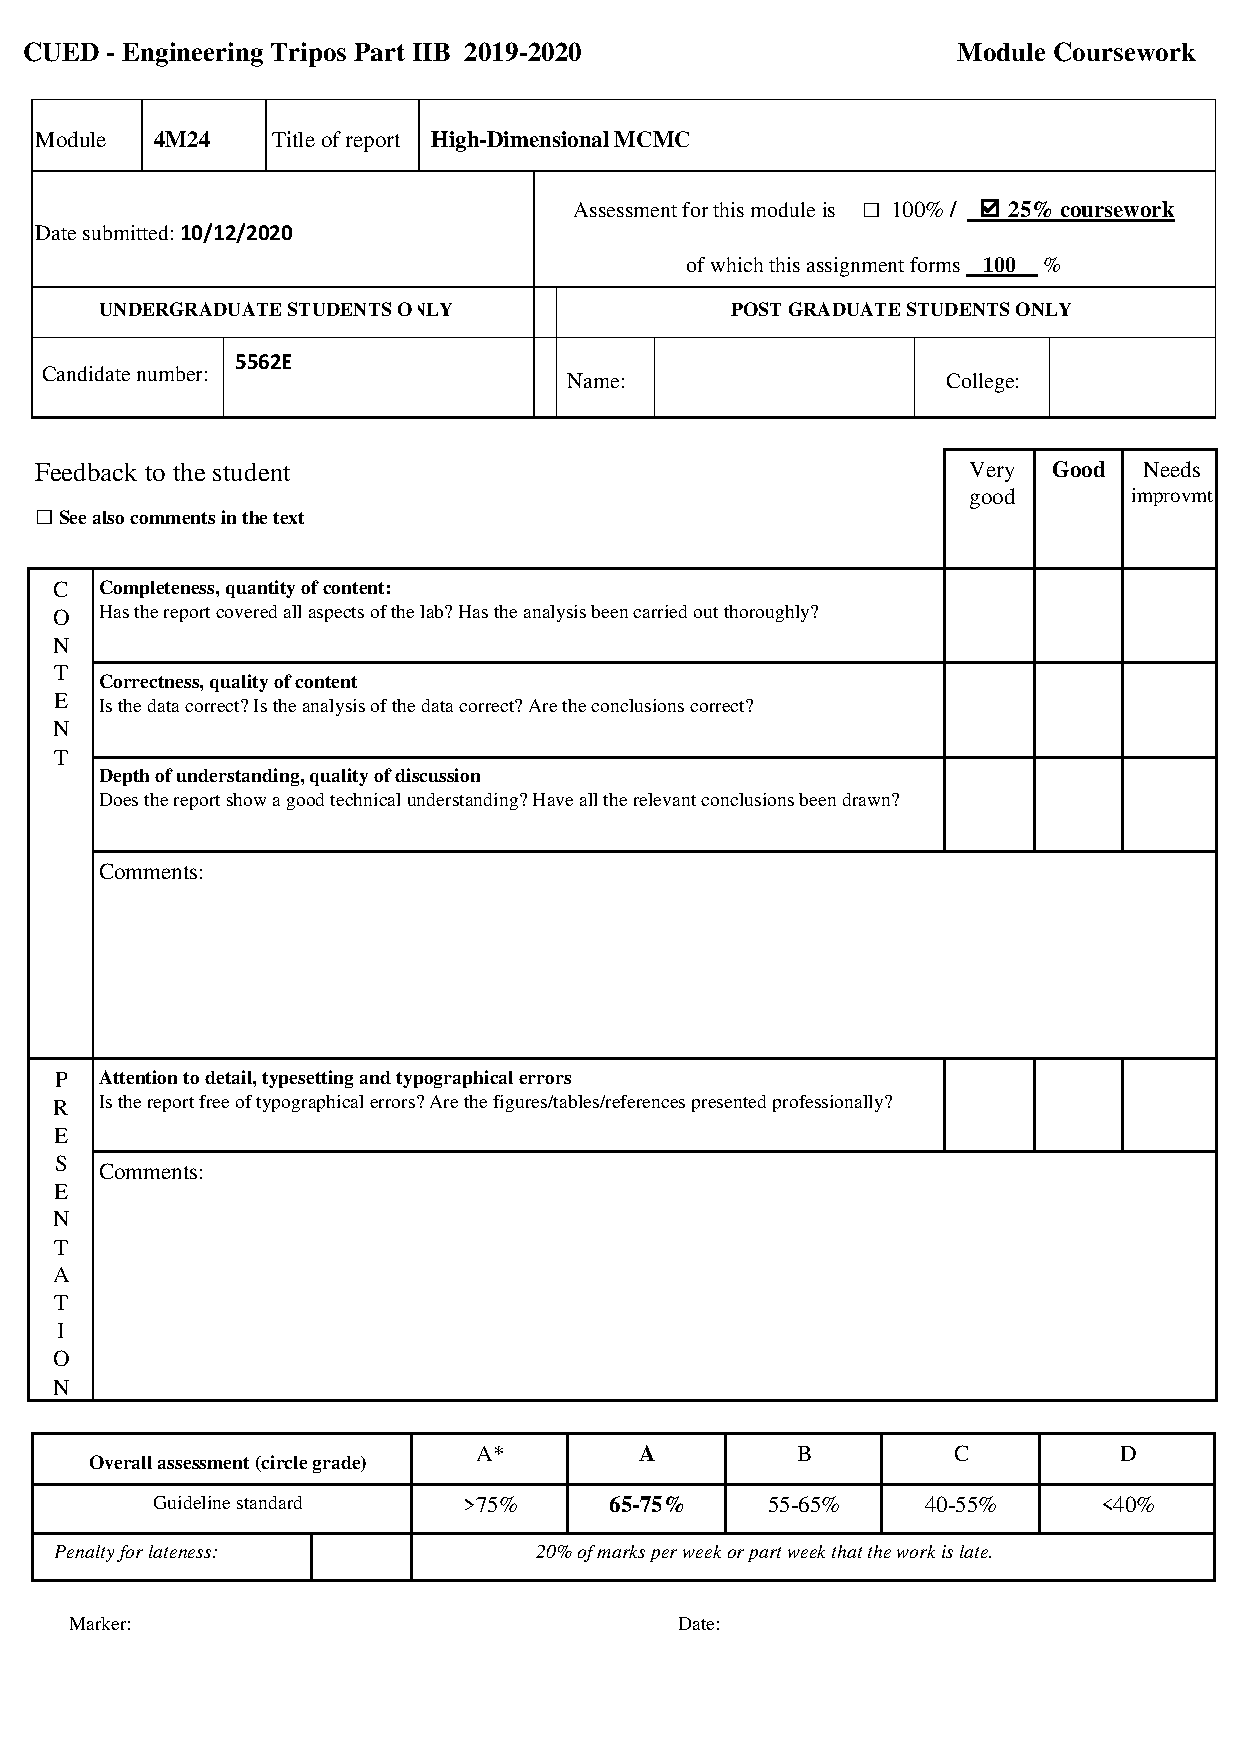
\includepdf[pages={1}]{4M24-Coversheet.pdf}

\setcounter{page}{1}
\maketitle

\begin{abstract}
	This report outlines the result of the 4M24 coursework on high-dimensional Markov Chain Monte Carlo (MCMC).
\end{abstract}

\tableofcontents

\section{Introduction}

\section{Simulation}
\subsection{Sampling from a Gaussian Process}

\textbf{Words}: XX

\end{document}
